\documentclass{article}
\setlength{\paperheight}{232.8mm}
\setlength{\paperwidth}{151.5mm}
\setlength\voffset{-26mm}
\setlength\hoffset{-32mm}

\bibliographystyle{plain}

\usepackage{pgfplots}
\usepgfplotslibrary{groupplots}
\pgfplotsset{compat=1.18}
\usepackage{longtable}
\usepackage{hyperref}
\usepackage{datetime}
\usepackage[capitalise,nameinlink]{cleveref}
\usepackage{booktabs}
\usepackage{caption}
\usepackage{subcaption}
\usepackage{ragged2e}
\begin{document}
\date{Compiled at {\ampmtime} on {\today}}
\title{Collaborative Model Optimization in Federated Stochastic Process Discovery: A Tool Report}
%\author{}
\maketitle
\section{Introduction}
This report summarizes the setup and results of a process discovery experiment conducted using the tool prepared for the paper titled “Collaborative Model Optimization in Federated Stochastic Process Discovery.” 
The following section outlines the discovery techniques used and their configurations in the experiment.
\Cref{sec:quality} specifies the evaluation criteria used to assess the quality of the discovered models and to compare the performance of the discovery techniques.
Finally, \cref{sec:results} presents the experimental results.
\section{Discovery}
The command line used to execute the experiment is listed below:
\begin{justify}
 -mspd -el "Hospital Billing - Event Log.xes"  m1  m2  m3 -p 50 -mxItr 20 -t 3600 -mms 1000 -pfs 100 -ebrm U - optm DFFA 
\end{justify}\noindent
\Cref{tbl:experiment} summarizes the key characteristics of the experimental setup used for performance comparison.
\begin{table}[h!] 
\centering 
\caption{Characteristics of the experiment} 
\label{tbl:experiment} 
\setlength{\tabcolsep}{6pt} % Adjust column spacing 
\fontsize{9}{11}\selectfont 
\begin{tabular}{@{}lr@{}} 
\toprule 
\textbf{Parameter} & \textbf{Value} \\ 
\midrule
Population size &50\\ 
Iterations &20\\ 
Time limit (s) &3600\\ 
Pareto front size &100\\ 
Maximum model size &1000\\ 
Optimized models &DFFA\\ 
Entropic relevance background model &U\\ 
Event log & \texttt{Hospital Billing - Event Log.xes} \\ 
Fitness coefficient $\alpha$ &0.0001 0.002 \\ 
Fitness Fuction &$\frac{\alpha}{size}+\frac{1-\alpha}{Er}$\\ 
Entropic relevance degradation threshold (tau) &0.09\\ 
\bottomrule 
\end{tabular}
\end{table} 
\noindent 

These discovery techniques are used in the experiment:
\begin{itemize}
\item GASPD ~\cite{Hanan2024};
\item FedGASPD ~\cite{zhian2025C};
\item OptFedGASPD;
\end{itemize}
\section{Quality}
\label{sec:quality}
The quality of the discovered models is assessed using two criteria: \emph{entropic relevance}, which captures stochastic precision and recall~\cite{AlkhammashPMG22}, and model \emph{size}, defined as the number of nodes and edges, which reflects model simplicity.

\section{Results}
\label{sec:results}
\Cref{fig:quality} presents the discovered deterministic frequency finite automata (DFFA) models with respect to entropic relevance and model size, where lower values are preferred for both criteria.
\begin{figure}[h!]
\centering
\begin{subfigure}[b]{0.99\textwidth}
\centering
\begin{tikzpicture}
\begin{axis}[ 
width=45mm, height=45mm,
xlabel={Entropic relevance}, 
ylabel={Size}, 
title={}, 
grid=both, 
ymin=0, ymax=13.1625, 
xmin=13.346729092092307, xmax=13.790424446528906,
tick label style={font=\footnotesize}, 
ylabel style={yshift=-5pt}, 
title style={yshift=-5pt}, 
legend style={at={(0.5,-0.3)}, anchor=north, legend columns=4, /tikz/every even column/.append }]
\addplot [scatter, only marks, point meta=explicit symbolic, scatter/classes={
OptFedGASPD={mark=*,red},
GASPD={mark=x,blue},
FedGASPD={mark=square,green}
}]
table [meta=label] {
 x           y     label 
13.515675029966893  13.0  OptFedGASPD
13.515675029966893  13.0  FedGASPD
13.62147850865432  13.0  GASPD
};
\legend{OptFedGASPD,GASPD,FedGASPD},
\end{axis}
\end{tikzpicture}
\caption{DFFA models}
\label{fig:quality:dffa}
\end{subfigure}
\caption{Discovered models plotted by size and entropic relevance for each representation type.}
\label{fig:quality}
\end{figure}

\noindent
\Cref{tbl:execution:time} reports the execution time (in iterations per second) for each input event log and method.
\begin{table}[h!]
\centering
\caption{Execution time comparison (iterations per second)}
\label{tbl:execution:time}
\setlength{\tabcolsep}{6pt}
\fontsize{8}{10}\selectfont
\begin{tabular}{lccc}
\toprule
Event log &OptFedGASPD&GASPD&FedGASPD\\
\midrule
Hospital Billing - Event Log.xes&274.15&687.95&274.15\\
\bottomrule
\end{tabular}
\end{table}
\begin{thebibliography}{9}
\bibitem{zhian2025B}
Hootan Zhian, Rajkumar Buyya, and Artem Polyvyanyy: \emph{Multi-Objective Metaheuristics for Effective and Efficient Stochastic Process Discovery}. Proceedings of the 23rd International Conference on Business Process Management (BPM) Seville, Spain, August 31–September 5, 2025.\bibitem{AlkhammashPMG22}
Hanan Alkhammash, Artem Polyvyanyy, Alistair Moffat, Luciano Garc{\'{\i}}a{-}Ba{\~{n}}uelos:\emph{Stochastic Directly-Follows Process Discovery Using Grammatical Inference}.Inf. Syst. 107: 101922 (2022)
\bibitem{Hanan2024}
Hanan Alkhammash, Artem Polyvyanyy, Alistair Moffat: \emph{Stochastic Directly-Follows Process Discovery Using Grammatical Inference}.  In: CAiSE, LNCS, vol. 14663, pp. 87–103, Springer (2024).\bibitem{zhian2025C}
Hootan Zhian, Rajkumar Buyya, and Artem Polyvyanyy: \emph{Federated Stochastic Process Discovery Using Gramatical Inference}.  In: CAiSE, LNCS, vol. 15702, pp. 76–93, Springer (2025).\end{thebibliography}
\appendix
\end{document}